\chapter{Графики FROC метрик}\label{sec:app:1}

В данном приложении приведены пять графиков FROC-метрик для сравнительного ананлиза бейслайн решения и предложенной модификации с аугментацией. Каждый график соответствует одному эксперименту из таблицы \ref{tab:result-metrics}

\begin{figure}[!h]
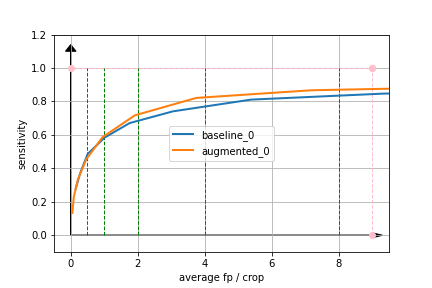
\includegraphics[width=\linewidth]{images/froc-results/cv_plot_0.png}
\caption{Итоговые FROC (over crop) кривые}\label{image:final-results-0}
\centering
\end{figure}

\begin{figure}[!h]
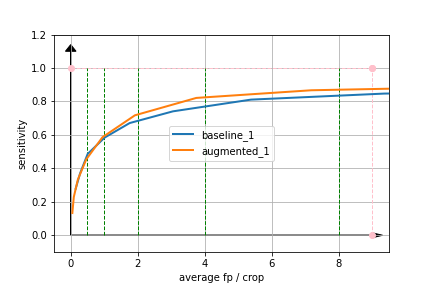
\includegraphics[width=\linewidth]{images/froc-results/cv_plot_1.png}
\caption{Итоговые FROC (over crop) кривые}\label{image:final-results-1}
\centering
\end{figure}

\begin{figure}[!h]
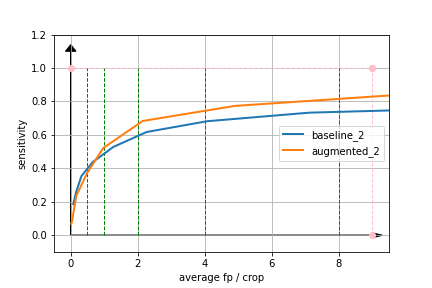
\includegraphics[width=\linewidth]{images/froc-results/cv_plot_2.png}
\caption{Итоговые FROC (over crop) кривые}\label{image:final-results-2}
\centering
\end{figure}

\begin{figure}[!h]
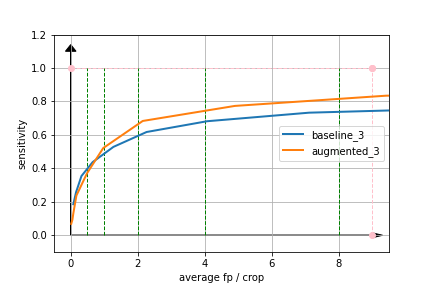
\includegraphics[width=\linewidth]{images/froc-results/cv_plot_3.png}
\caption{Итоговые FROC (over crop) кривые}\label{image:final-results-3}
\centering
\end{figure}

\begin{figure}[!h]
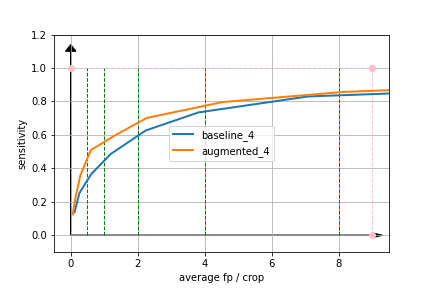
\includegraphics[width=\linewidth]{images/froc-results/cv_plot_4.png}
\caption{Итоговые FROC (over crop) кривые}\label{image:final-results-4}
\centering
\end{figure}